\documentclass[12pt, a4paper]{book}
\usepackage[T1]{fontenc}
\usepackage[utf8]{inputenc}
\usepackage[charter, cal=cmcal]{mathdesign}
\usepackage[scaled=0.92]{helvet}
\usepackage{geometry}
\geometry{a4paper, top=30mm, bottom=30mm, inner=32mm, outer=25mm}
\usepackage{amsmath, amssymb}
\usepackage[version=4]{mhchem}
\usepackage[dvipsnames,svgnames,table]{xcolor}
\usepackage{tikz}
\usetikzlibrary{arrows.meta, positioning, calc, backgrounds, shapes.geometric}
\usepackage{tcolorbox}
\tcbuselibrary{skins, breakable}
\usepackage{titlesec}
\usepackage{fancyhdr}
\usepackage{enumitem}
\usepackage{booktabs}
\usepackage{array}
\usepackage{parskip}
\usepackage{siunitx}
\usepackage[colorlinks=true, linkcolor=BrickRed, urlcolor=NavyBlue]{hyperref}

\definecolor{JourneyColor}{HTML}{1A5276}
\definecolor{ModuleColor}{HTML}{2E86C1}
\definecolor{PuzzleColor}{HTML}{145A32}
\definecolor{DiscoveryColor}{HTML}{B7950B}
\definecolor{WarningColor}{HTML}{C0392B}
\definecolor{ProblemColor}{HTML}{4A235A}
\definecolor{ReflectColor}{HTML}{117A65}
\definecolor{HistoryColor}{HTML}{6E2F1A}
\definecolor{BondColor}{HTML}{1A5276}
\definecolor{LPColor}{HTML}{922B21}

\newtcolorbox{puzzlebox}[1][]{enhanced,breakable,
  colback=PuzzleColor!6,colframe=PuzzleColor,fonttitle=\bfseries\sffamily,
  title={The Puzzle},attach boxed title to top left={yshift=-2mm,xshift=6mm},
  boxed title style={colback=PuzzleColor},borderline west={3pt}{0pt}{PuzzleColor},#1}
\newtcolorbox{discoverybox}[1][]{enhanced,breakable,
  colback=DiscoveryColor!8,colframe=DiscoveryColor,fonttitle=\bfseries\sffamily,
  title={Discovery},attach boxed title to top left={yshift=-2mm,xshift=6mm},
  boxed title style={colback=DiscoveryColor},borderline west={3pt}{0pt}{DiscoveryColor},#1}
\newtcolorbox{problembox}[1][]{enhanced,breakable,
  colback=ProblemColor!5,colframe=ProblemColor,fonttitle=\bfseries\sffamily,
  title={Problems},attach boxed title to top left={yshift=-2mm,xshift=6mm},
  boxed title style={colback=ProblemColor},borderline west={3pt}{0pt}{ProblemColor},#1}
\newtcolorbox{deepbox}[1][]{enhanced,breakable,
  colback=JourneyColor!5,colframe=JourneyColor,fonttitle=\bfseries\sffamily,
  title={Deep Problems},attach boxed title to top left={yshift=-2mm,xshift=6mm},
  boxed title style={colback=JourneyColor},borderline west={4pt}{0pt}{JourneyColor},#1}
\newtcolorbox{reflectionbox}[1][]{enhanced,breakable,
  colback=ReflectColor!6,colframe=ReflectColor,fonttitle=\bfseries\sffamily,
  title={Reflection},attach boxed title to top left={yshift=-2mm,xshift=6mm},
  boxed title style={colback=ReflectColor},borderline west={3pt}{0pt}{ReflectColor},#1}
\newtcolorbox{namedconcept}[2][]{enhanced,
  colback=ModuleColor!6,colframe=ModuleColor,fonttitle=\bfseries\sffamily\large,
  title={#2},attach boxed title to top left={yshift=-2mm,xshift=6mm},
  boxed title style={colback=ModuleColor},#1}
\newtcolorbox{modelbreaks}[1][]{enhanced,breakable,
  colback=WarningColor!6,colframe=WarningColor,fonttitle=\bfseries\sffamily,
  title={Where This Model Breaks},attach boxed title to top left={yshift=-2mm,xshift=6mm},
  boxed title style={colback=WarningColor},borderline west={4pt}{0pt}{WarningColor},#1}

\titleformat{\chapter}[display]
  {\normalfont\sffamily\huge\bfseries\color{JourneyColor}}
  {\textcolor{JourneyColor!60}{\chaptertitlename\ \thechapter}}{10pt}{\Huge}
  [\vspace{2pt}\textcolor{JourneyColor}{\titlerule[1.5pt]}]
\titleformat{\section}{\normalfont\sffamily\Large\bfseries\color{ModuleColor}}
  {\thesection}{1em}{}[\textcolor{ModuleColor!40}{\titlerule[0.6pt]}]
\titleformat{\subsection}{\normalfont\sffamily\large\bfseries\color{JourneyColor!80}}
  {\thesubsection}{1em}{}
\pagestyle{fancy}\fancyhf{}
\fancyhead[LE]{\small\sffamily\textcolor{JourneyColor}{\leftmark}}
\fancyhead[RO]{\small\sffamily\textcolor{ModuleColor}{\rightmark}}
\fancyfoot[C]{\small\thepage}
\renewcommand{\headrulewidth}{0.4pt}
\newcommand{\newterm}[1]{\textit{\textcolor{DiscoveryColor}{#1}}}

\begin{document}
\setcounter{chapter}{3}
\chapter[Journey 4 --- The Bond]{Journey Four\\[8pt]
  \textcolor{ModuleColor}{\large The Bond: Why Atoms Stick Together}}
\setcounter{section}{3}

\section{Module 4.4 --- Molecular Shape: VSEPR and Beyond}

\subsection*{Motivation}

The shape of a molecule determines nearly everything
about its physical properties and chemical behaviour:
whether it is polar or nonpolar,
whether it fits into an enzyme active site,
whether it can hydrogen-bond,
what boiling point it has,
and how it reacts.

Water is bent ($104.5^\circ$) and polar.
Carbon dioxide is linear and nonpolar.
The difference in properties --- water is liquid at room temperature,
\ce{CO2} is a gas --- traces directly to this shape difference.

This module builds the framework for predicting molecular shape
from Lewis structures, explains the quantitative basis for
bond angle variations, and shows where simple models fail.

\subsection{VSEPR: The Central Idea}

\newterm{Valence Shell Electron Pair Repulsion (VSEPR)} theory
rests on one principle:

\begin{namedconcept}{The VSEPR Principle}
Electron pairs in the valence shell of a central atom
arrange themselves to minimise repulsion.
This means they occupy positions as far apart as possible.

The geometry of electron pairs (the \newterm{electron geometry})
determines the molecular geometry (the shape defined by
bonded atoms only).

Repulsion order: lone pair--lone pair $>$ lone pair--bond pair
$>$ bond pair--bond pair.

Lone pairs occupy more angular space than bonding pairs
and compress bond angles.
\end{namedconcept}

\begin{center}
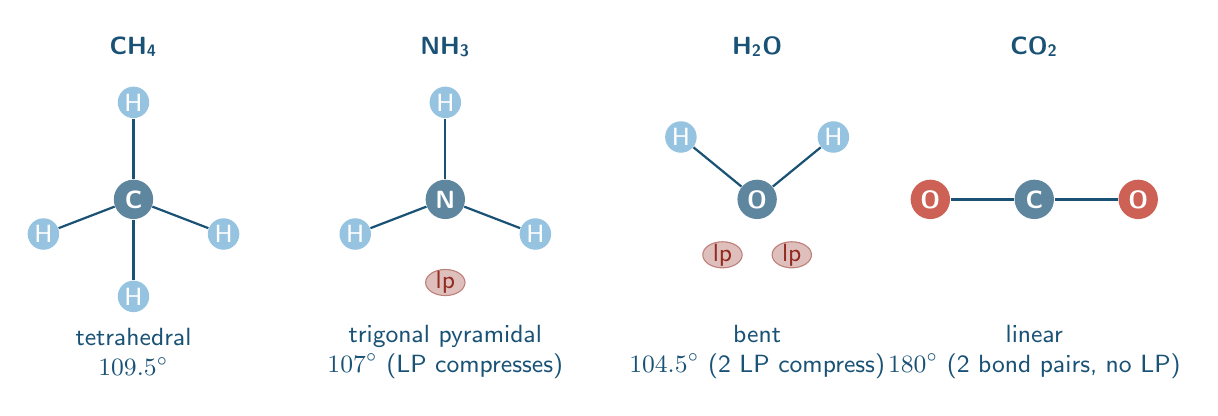
\begin{tikzpicture}[
  every node/.style={font=\sffamily\small, align=center},
  atom/.style={circle, fill=JourneyColor!70, minimum size=0.5cm,
               inner sep=0, text=white, font=\sffamily\small\bfseries},
  hatom/.style={circle, fill=ModuleColor!50, minimum size=0.4cm,
                inner sep=0, text=white, font=\sffamily\small},
  lp/.style={ellipse, fill=LPColor!30, draw=LPColor!60,
             minimum width=0.5cm, minimum height=0.3cm},
  scale=0.88
]

% ── CH4 tetrahedral ──────────────────────────────────────────────────────────
\begin{scope}[xshift=0cm]
  \node[atom] (C) at (0,0) {C};
  \node[hatom] (H1) at (0, 1.4) {H};
  \node[hatom] (H2) at (1.3,-0.5) {H};
  \node[hatom] (H3) at (-1.3,-0.5) {H};
  \node[hatom] (H4) at (0,-1.4) {H};
  \foreach \h in {H1,H2,H3,H4} {
    \draw[thick, BondColor] (C) -- (\h);
  }
  \node[font=\sffamily\small\bfseries, color=JourneyColor]
    at (0, 2.2) {\ce{CH4}};
  \node[font=\sffamily\small, color=JourneyColor]
    at (0,-2.2) {tetrahedral\\$109.5^\circ$};
\end{scope}

% ── NH3 trigonal pyramidal ───────────────────────────────────────────────────
\begin{scope}[xshift=4.5cm]
  \node[atom] (N) at (0,0) {N};
  \node[hatom] (H1) at (0, 1.4) {H};
  \node[hatom] (H2) at (1.3,-0.5) {H};
  \node[hatom] (H3) at (-1.3,-0.5) {H};
  \node[lp] at (0,-1.2) {};
  \node[font=\sffamily\small, color=LPColor] at (0,-1.2) {lp};
  \foreach \h in {H1,H2,H3} {
    \draw[thick, BondColor] (N) -- (\h);
  }
  \node[font=\sffamily\small\bfseries, color=JourneyColor]
    at (0, 2.2) {\ce{NH3}};
  \node[font=\sffamily\small, color=JourneyColor]
    at (0,-2.2) {trigonal pyramidal\\$107^\circ$ (LP compresses)};
\end{scope}

% ── H2O bent ──────────────────────────────────────────────────────────────────
\begin{scope}[xshift=9.0cm]
  \node[atom] (O) at (0,0) {O};
  \node[hatom] (H1) at (1.1, 0.9) {H};
  \node[hatom] (H2) at (-1.1, 0.9) {H};
  \node[lp] at (0.5,-0.8) {};
  \node[font=\sffamily\small, color=LPColor] at (0.5,-0.8) {lp};
  \node[lp] at (-0.5,-0.8) {};
  \node[font=\sffamily\small, color=LPColor] at (-0.5,-0.8) {lp};
  \foreach \h in {H1,H2} {
    \draw[thick, BondColor] (O) -- (\h);
  }
  \node[font=\sffamily\small\bfseries, color=JourneyColor]
    at (0, 2.2) {\ce{H2O}};
  \node[font=\sffamily\small, color=JourneyColor]
    at (0,-2.2) {bent\\$104.5^\circ$ (2 LP compress)};
\end{scope}

% ── CO2 linear ────────────────────────────────────────────────────────────────
\begin{scope}[xshift=13.0cm]
  \node[atom] (C) at (0,0) {C};
  \node[atom, fill=WarningColor!80] (O1) at (-1.5,0) {O};
  \node[atom, fill=WarningColor!80] (O2) at (1.5,0) {O};
  \draw[very thick, BondColor] (C) -- (O1);
  \draw[very thick, BondColor] (C) -- (O2);
  \node[font=\sffamily\small\bfseries, color=JourneyColor]
    at (0, 2.2) {\ce{CO2}};
  \node[font=\sffamily\small, color=JourneyColor]
    at (0,-2.2) {linear\\$180^\circ$ (2 bond pairs, no LP)};
\end{scope}

\end{tikzpicture}
\end{center}

\vspace{0.4em}

The sequence \ce{CH4} ($109.5^\circ$) $\to$ \ce{NH3} ($107^\circ$)
$\to$ \ce{H2O} ($104.5^\circ$) beautifully illustrates
the progressive compression by lone pairs.
Each additional lone pair reduces the bond angle by
about $2.5^\circ$.

\subsection{The Full VSEPR Table}

\begin{center}
\small
\begin{tabular}{cclllp{3.5cm}}
\toprule
Electron pairs & Lone pairs & Electron geometry & Molecular geometry & Bond angle & Example \\
\midrule
2 & 0 & linear          & linear          & $180^\circ$ & \ce{BeCl2}, \ce{CO2} \\
3 & 0 & trigonal planar & trigonal planar & $120^\circ$ & \ce{BF3}, \ce{SO3} \\
3 & 1 & trigonal planar & bent            & $<120^\circ$ & \ce{SO2}, \ce{O3} \\
4 & 0 & tetrahedral     & tetrahedral     & $109.5^\circ$ & \ce{CH4}, \ce{SiCl4} \\
4 & 1 & tetrahedral     & trigonal pyr.   & $107^\circ$ & \ce{NH3}, \ce{PCl3} \\
4 & 2 & tetrahedral     & bent            & $104.5^\circ$ & \ce{H2O}, \ce{H2S} \\
5 & 0 & trig.\ bipyramidal & trig.\ bipyramidal & $90/120^\circ$ & \ce{PCl5}, \ce{PF5} \\
5 & 1 & trig.\ bipyramidal & see-saw       & $<90/120^\circ$ & \ce{SF4} \\
5 & 2 & trig.\ bipyramidal & T-shaped      & $<90^\circ$ & \ce{ClF3} \\
5 & 3 & trig.\ bipyramidal & linear        & $90^\circ$ & \ce{XeF2} \\
6 & 0 & octahedral      & octahedral      & $90^\circ$ & \ce{SF6}, \ce{PF6-} \\
6 & 1 & octahedral      & square pyramidal & $<90^\circ$ & \ce{IF5}, \ce{BrF5} \\
6 & 2 & octahedral      & square planar   & $90^\circ$ & \ce{XeF4}, \ce{ICl4-} \\
\bottomrule
\end{tabular}
\end{center}

\subsection{Polarity: Shape Determines Dipole Moment}

A molecule is polar if it has a net \newterm{dipole moment}
$\vec{\mu}$ --- a separation of positive and negative charge
centres.
The dipole moment is the vector sum of all bond dipoles.

Shape determines polarity in crucial ways:

\begin{center}
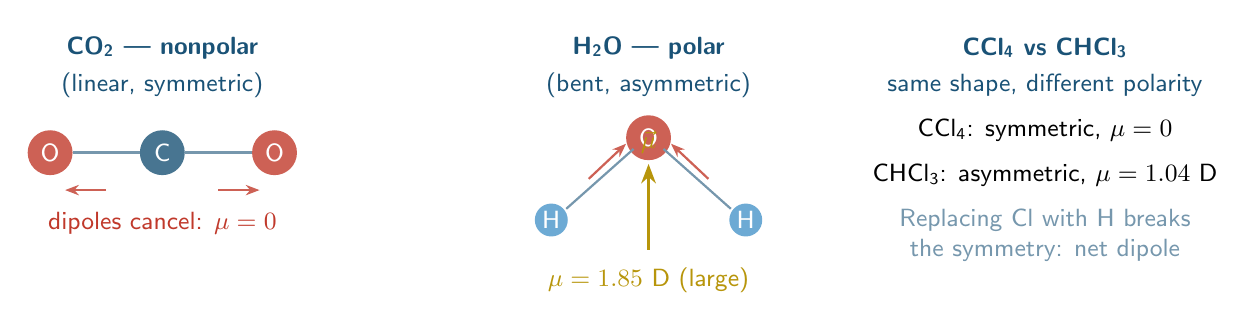
\begin{tikzpicture}[every node/.style={font=\sffamily\small}, scale=0.95]

  % CO2: linear, symmetric, nonpolar
  \begin{scope}[xshift=0cm]
    \node[font=\sffamily\small\bfseries, color=JourneyColor]
      at (1.5, 2.2) {\ce{CO2} --- nonpolar};
    \node[font=\sffamily\small, color=JourneyColor]
      at (1.5, 1.7) {(linear, symmetric)};
    % atoms
    \fill[WarningColor!80] (0,0.8) circle (0.3cm);
    \node[font=\sffamily\small, text=white] at (0,0.8) {O};
    \fill[JourneyColor!80] (1.5,0.8) circle (0.3cm);
    \node[font=\sffamily\small, text=white] at (1.5,0.8) {C};
    \fill[WarningColor!80] (3.0,0.8) circle (0.3cm);
    \node[font=\sffamily\small, text=white] at (3.0,0.8) {O};
    \draw[very thick, JourneyColor!60] (0.3,0.8)--(1.2,0.8);
    \draw[very thick, JourneyColor!60] (1.8,0.8)--(2.7,0.8);
    % Bond dipoles cancel
    \draw[-{Stealth[length=5pt]}, thick, WarningColor!80]
      (0.75,0.3) -- (0.2,0.3);
    \draw[-{Stealth[length=5pt]}, thick, WarningColor!80]
      (2.25,0.3) -- (2.8,0.3);
    \node[font=\sffamily\small, color=WarningColor]
      at (1.5,-0.15) {dipoles cancel: $\mu = 0$};
  \end{scope}

  % H2O: bent, asymmetric, polar
  \begin{scope}[xshift=6.5cm]
    \node[font=\sffamily\small\bfseries, color=JourneyColor]
      at (1.5, 2.2) {\ce{H2O} --- polar};
    \node[font=\sffamily\small, color=JourneyColor]
      at (1.5, 1.7) {(bent, asymmetric)};
    % atoms
    \fill[WarningColor!80] (1.5,1.0) circle (0.3cm);
    \node[font=\sffamily\small, text=white] at (1.5,1.0) {O};
    \fill[ModuleColor!70] (0.2,-0.1) circle (0.22cm);
    \node[font=\sffamily\small, text=white] at (0.2,-0.1) {H};
    \fill[ModuleColor!70] (2.8,-0.1) circle (0.22cm);
    \node[font=\sffamily\small, text=white] at (2.8,-0.1) {H};
    \draw[thick, JourneyColor!60] (0.4,0.05)--(1.3,0.85);
    \draw[thick, JourneyColor!60] (2.6,0.05)--(1.7,0.85);
    % Bond dipoles and net dipole
    \draw[-{Stealth[length=5pt]}, thick, WarningColor!80]
      (0.7,0.45) -- (1.2,0.92);
    \draw[-{Stealth[length=5pt]}, thick, WarningColor!80]
      (2.3,0.45) -- (1.8,0.92);
    \draw[-{Stealth[length=7pt]}, very thick, DiscoveryColor]
      (1.5,-0.5) -- (1.5,0.65)
      node[above, font=\sffamily\small, text=DiscoveryColor] {$\vec{\mu}$};
    \node[font=\sffamily\small, color=DiscoveryColor]
      at (1.5,-0.9) {$\mu = 1.85$ D (large)};
  \end{scope}

  % CCl4 vs CHCl3
  \begin{scope}[xshift=12.5cm]
    \node[font=\sffamily\small\bfseries, color=JourneyColor]
      at (0.8, 2.2) {\ce{CCl4} vs \ce{CHCl3}};
    \node[font=\sffamily\small, color=JourneyColor]
      at (0.8,1.7) {same shape, different polarity};
    \node[font=\sffamily\small] at (0.8,1.1)
      {\ce{CCl4}: symmetric, $\mu = 0$};
    \node[font=\sffamily\small] at (0.8,0.5)
      {\ce{CHCl3}: asymmetric, $\mu = 1.04$ D};
    \node[font=\sffamily\small, text=JourneyColor!60] at (0.8,-0.1)
      {Replacing Cl with H breaks};
    \node[font=\sffamily\small, text=JourneyColor!60] at (0.8,-0.5)
      {the symmetry: net dipole};
  \end{scope}

\end{tikzpicture}
\end{center}

\vspace{0.4em}

Key consequences of polarity:
\begin{itemize}[nosep, leftmargin=2em]
  \item Polar molecules have higher boiling points
        (stronger intermolecular forces).
  \item Polar molecules are soluble in polar solvents
        (water); nonpolar ones in nonpolar solvents.
  \item Molecular polarity determines whether a molecule
        can rotate in a microwave field (basis of
        microwave spectroscopy and microwave ovens).
\end{itemize}

\subsection{Beyond VSEPR: Why Are Bond Angles Not Exactly Predicted?}

VSEPR predicts qualitative geometry well, but quantitative
bond angles require accounting for several additional factors.

\subsubsection{Electronegativity of Substituents}

More electronegative substituents pull electron density
away from the central atom, making the bonding pair
more compact and reducing its repulsion --- allowing
other bond angles to open.

For the series \ce{NH3} ($107^\circ$), \ce{PH3} ($93.5^\circ$),
\ce{AsH3} ($91.8^\circ$), \ce{SbH3} ($91.3^\circ$):
the angles approach $90^\circ$ down the group because the
$p$ orbitals become progressively less hybridised
(nearly pure $p$--$p$ overlap), and $p$ orbitals are
perpendicular.

\subsubsection{Multiple Bonds}

Double bonds occupy more angular space than single bonds
(two electron pairs in a bonding region).
This causes compression of adjacent single bonds.

In \ce{SO2} (which has one double bond and one lone pair
on S): the bond angle is $119^\circ$, close to $120^\circ$
for the double bond side but compressed by the lone pair.

\subsubsection{VSEPR for Expanded Octets}

For 5-coordinate molecules (trigonal bipyramidal), VSEPR
predicts lone pairs prefer equatorial positions
(three equal $120^\circ$ neighbours rather than two
$90^\circ$ and three $120^\circ$ axial neighbours).
This correctly predicts the structure of \ce{SF4} (see-saw).

\begin{problembox}
\begin{enumerate}[label=\textbf{\arabic*.}]
  \item \textbf{VSEPR predictions.}
    For each of the following, draw the Lewis structure,
    determine the number of bond pairs and lone pairs,
    and predict the molecular geometry and approximate bond angle(s):
    \begin{enumerate}[label=(\alph*)]
      \item \ce{PF3}
      \item \ce{IF3}
      \item \ce{ClF3}
      \item \ce{XeF4}
      \item \ce{ICl4-}
      \item \ce{SF4}
    \end{enumerate}

  \item \textbf{Polarity analysis.}
    \begin{enumerate}[label=(\alph*)]
      \item Explain why \ce{BF3} ($D_{3h}$ symmetry) is
            nonpolar even though each B--F bond is polar.
      \item \ce{NF3} and \ce{NH3} have similar shapes but
            very different dipole moments:
            \ce{NH3} $\mu = 1.47$ D; \ce{NF3} $\mu = 0.24$ D.
            The B--F bond dipoles point toward N (N is less
            electronegative than F).
            In \ce{NH3}, the N--H bond dipoles and the lone
            pair on N both point in the same direction.
            In \ce{NF3}, the lone pair and bond dipoles point
            in opposite directions.
            Explain the dramatic difference in $\mu$ using
            vector addition of bond dipoles.
      \item Is \ce{cis}-\ce{CHCl=CHCl} or \ce{trans}-\ce{CHCl=CHCl}
            expected to be more polar? Explain.
    \end{enumerate}

  \item \textbf{Molecular shape and physical properties.}
    \begin{enumerate}[label=(\alph*)]
      \item Water (b.p. $100^\circ$C) and hydrogen sulphide
            (b.p. $-60^\circ$C) are both bent with similar
            bond angles.
            List the intermolecular forces present in each.
            Why does water have such a dramatically higher
            boiling point?
      \item \ce{cis}-but-2-ene (b.p. $4^\circ$C) has a dipole
            moment; \ce{trans}-but-2-ene (b.p. $1^\circ$C)
            does not.
            Yet their boiling points differ by only $3^\circ$C.
            What does this tell us about the relative strengths
            of dipole-dipole forces versus London dispersion
            forces for these molecules?
    \end{enumerate}
\end{enumerate}
\end{problembox}

\subsection*{Where VSEPR Breaks Down}

\begin{modelbreaks}
\begin{itemize}[nosep, leftmargin=2em]
  \item \textbf{Transition metal compounds.}
        VSEPR applies to main-group elements.
        For transition metals, $d$ orbital geometry
        and crystal field effects dominate.
        \ce{[PtCl4]^{2-}} is square planar
        (not tetrahedral as VSEPR predicts for 4 ligands).

  \item \textbf{Heavy main-group compounds.}
        \ce{PbCl2} (2 bonds, 1 lone pair) should be bent
        by VSEPR.
        It is actually nearly linear in the gas phase:
        the lone pair is ``inert'' due to relativistic
        effects stabilising the $6s^2$ pair
        (the ``inert pair effect'').

  \item \textbf{Resonance structures.}
        Ozone (\ce{O3}) has two resonance structures.
        VSEPR treats it as having a double bond and a lone pair
        (which is formally correct for one structure),
        but the true geometry comes from the delocalised
        $\pi$ system, not from VSEPR.

  \item \textbf{Molecules with no lone pairs on central atom
        but extreme steric effects.}
        Very large substituents can distort geometry
        significantly beyond VSEPR predictions.
        Di-tert-butyl ether has an O--C--O angle much
        larger than $109.5^\circ$ due to steric repulsion.
\end{itemize}
\end{modelbreaks}

\subsection*{Deep Problems}

\begin{deepbox}
\begin{enumerate}[label=\textbf{D\arabic*.}]

  \item \textbf{The geometry of the ribosome active site.}

    The ribosome catalyses peptide bond formation:
    the amine group of one amino acid attacks the
    carbonyl carbon of another in a tetrahedral transition state.

    \begin{enumerate}[label=(\alph*)]
      \item The carbonyl carbon in a peptide bond (\ce{C=O})
            is $sp^2$ hybridised.
            Draw its geometry and state the bond angles.
      \item During the reaction, the carbon becomes
            $sp^3$ hybridised (tetrahedral intermediate).
            Describe the geometric change at the carbon.
      \item The ribosome must accommodate this geometric
            change in its active site.
            Using VSEPR, predict the approximate geometry
            of the transition state carbon.
      \item Enzyme active sites are ``pre-organised'' to
            stabilise the transition state geometry.
            What does this mean in terms of the complementarity
            between the enzyme shape and the transition
            state shape?
    \end{enumerate}

  \item \textbf{Molecular symmetry and spectroscopy.}

    Infrared (IR) spectroscopy detects vibrational modes
    of molecules.
    A vibration is IR-active only if it changes the
    dipole moment of the molecule.

    \begin{enumerate}[label=(\alph*)]
      \item \ce{CO2} is linear and nonpolar.
            It has three vibrational modes: symmetric stretch,
            asymmetric stretch, and two degenerate bends.
            Which are IR-active? Explain using dipole change.
      \item \ce{H2O} is bent and polar.
            All three of its vibrational modes are IR-active.
            Does this mean every vibration of a polar molecule
            must be IR-active? Explain.
      \item \ce{N2} and \ce{O2} are not IR-active.
            \ce{CO} is IR-active.
            Explain the difference.
      \item The atmosphere of Venus is $\sim$96\% \ce{CO2}.
            Explain, using the concept of IR-active vibrational
            modes and the greenhouse effect, why Venus has
            a surface temperature of $\sim\SI{465}{\degreeCelsius}$.
    \end{enumerate}

\end{enumerate}
\end{deepbox}

\subsection*{Reflection}

\begin{reflectionbox}
\begin{enumerate}[label=\textbf{R\arabic*.}]
  \item VSEPR is a geometric model with no quantum mechanics.
    It doesn't explain \emph{why} electrons repel each other ---
    it just asserts that they do and asks what geometry minimises this.
    \textbf{Can a model be scientifically useful without
    being mechanistically grounded?}
    What kind of understanding does VSEPR give us?

  \item The shape of water ($104.5^\circ$ instead of the
    ``ideal'' $109.5^\circ$) is caused by lone pair repulsion.
    That $5^\circ$ difference means water can form a
    three-dimensional hydrogen-bonded network, giving it
    anomalously high boiling point, surface tension, and
    the property of expanding on freezing (crucial for life).
    \textbf{Trace the chain of consequences: the bond angle
    of water determines the existence of ice floating
    rather than sinking.}
    What does it mean that a small geometric detail
    has such large-scale consequences?

  \item Molecular shape is the basis of the ``lock and key''
    model of enzyme catalysis.
    \textbf{Is molecular recognition a physical phenomenon
    (shape complementarity, electrostatics)
    or something more?}
    What is the relationship between molecular shape and
    biological function?
\end{enumerate}
\end{reflectionbox}

\vspace{1.5em}
\begin{center}
\begin{tcolorbox}[enhanced, colback=DiscoveryColor!8, colframe=DiscoveryColor,
  width=0.88\textwidth, arc=3pt]
\centering\sffamily\small
\textbf{What we invented in this module.}\\[4pt]
Molecular shape follows from one principle: electron pairs
arrange to minimise repulsion.
Lone pairs compress bond angles; multiple bonds take more
space than single bonds; electronegativity tunes the
quantitative angles.
Shape determines polarity, and polarity determines physical
properties: boiling point, solubility, biological activity.
The $5^\circ$ difference between the tetrahedral ideal
($109.5^\circ$) and the water bond angle ($104.5^\circ$)
is directly responsible for the hydrogen-bonding network
that makes water the solvent of life.
\end{tcolorbox}
\end{center}

\vspace{2em}
\noindent\textcolor{JourneyColor!40}{\rule{\textwidth}{0.6pt}}
\begin{center}\textit{\sffamily\small
Module 4.4 complete. Continue to Module 4.5:\\
\textbf{Intermolecular Forces: Between Molecules}.}
\end{center}
\end{document}